\RequirePackage{plautopatch}
\RequirePackage[l2tabu, orthodox]{nag}

\documentclass[platex,dvipdfmx]{jlreq}			% for platex
% \documentclass[uplatex,dvipdfmx]{jlreq}		% for uplatex
\usepackage{graphicx}
\usepackage{bxtexlogo}
\usepackage{booktabs}
\usepackage{array}
\usepackage{amsmath}
\usepackage{xcolor}
\usepackage{hyperref} 
\usepackage{amsfonts}
\usepackage{caption}   % キャプションを調整するパッケージ
\usepackage{physics} % package for making some command easier, such as "\qty", "\dd", "\pdv", "\vb", "\mqty", "\braket"
\usepackage{svg}

\author{齊藤孝太朗}
\date{\today}
\begin{document}

\thispagestyle{empty}

\vspace*{1cm}

\begin{center}
    \huge 修士論文
\end{center}

\vspace{3cm}

\begin{center}
    \LARGE
    オルソパラ転換レートの温度依存性
\end{center}

\vspace{4cm}

\begin{center}
    \Large
    指導教員 吉岡 孝高 准教授
\end{center}

\vspace{3cm}

\begin{center}
    \Large
    令和8年1月提出
\end{center}

\vspace{2cm}

\begin{center}
    \Large
    東京大学工学系研究科物理工学専攻\\
    37-246618 齊藤 孝太朗
\end{center}


\newpage
\begin{abstract}
The yellow 1s excitons in a cuprous oxide \(\mathrm{Cu_2O}\) crystal are split into two distinct states depending on the spin configuration: a triply degenerate orthoexciton state and a singly degenerate paraexciton state. Because 1s paraexciton is pure spin triplet state, paraexcitons interact weakly with the radiative field and thus exhibit long lifetimes. Typically, paraexcitons are generated from optically accessible orthoexcitons via an ortho-to-para conversion process. Owing to their long lifetimes, paraexcitons have attracted attention as a candidate for exciton Bose-Einstein condensation (BEC). To investigate the characteristics of a condensate and the kinetics of orthoexcitons and paraexcitons, it is crucial to analyze the ortho-to-para conversion process, which determines the time scales of paraexciton generation.

In this presentation, we review the temperature dependence of the ortho-to-para conversion rate measured at temperatures ranging from 2 K to 20 K. We also present a conversion model that explains experimental results, based on transverse acoustic (TA) phonon scattering [1]. Furthermore, we present the latest results from our group on measurements of the ortho-to-para conversion rate at sub-Kelvin temperatures and validate the proposed conversion model against the experimental data taken at sub-Kelvin temperatures.
\end{abstract}
\newpage
\tableofcontents
\newpage
本論文で使用する主要な記号およびシンボルは以下の通りである。

\begin{table}[h]
    \centering
    \begin{tabular}{|c|m{8cm}|c|}
        \hline
        記号 & 意味・定義 & 単位 \\ \hline
        \( h \) & プランク定数 & \( \mathrm{J \cdot s} \) \\ \hline
        \( \hbar \) & 剣幕プランク定数 (\( \hbar = \frac{h}{2\pi} \)) & \( \mathrm{J \cdot s} \) \\ \hline
        \( E \) & エネルギー & \( \mathrm{J} \) \\ \hline
        \( \nu \) & 周波数 & \( \mathrm{Hz} \) \\ \hline
        \( \lambda \) & 波長 & \( \mathrm{m} \) \\ \hline
        \( k_B \) & ボルツマン定数 & \( \mathrm{J/K} \) \\ \hline
        \( m \) & 質量 & \( \mathrm{kg} \) \\ \hline
        \vdots & \vdots & \vdots \\ \hline
    \end{tabular}
    \caption{記号一覧}
    \label{tab:symbol_list}
\end{table}
\newpage
% chapter1.tex
\newpage
\section{序論}
\renewcommand{\thefigure}{\thesection-\arabic{figure}}
\subsection{研究の背景}
直接遷移型半導体である亜酸化銅結晶の励起子はその長寿命の性質から長年励起子BECの候補として注目されてきた。
\subsection{研究の目的}
励起子のオルソパラ転換レートの測定を行った。
応力が印加された亜酸化銅バルク結晶に、黄色系列1sオルソ励起子のフォノンサイドバンド吸収に対応する波長の可視光を照射することで光生成されたと、バルク内で光生成された黄色系列1sオルソ励起子は、より低いエネルギー準位に位置するは黄色系列1sパラ励起子へ転換する。
先行研究では、オルソ励起子からパラ励起子への転換レートは2 K以上の温度領域での報告にとどまり、サブケルビン温度領域では未解明であった。
今回の実験では結晶の冷却に希釈冷凍機を用いて、サブケルビン温度領域でのオルソーパラ転換レートの測定を初めて行い、転換レートの温度依存性を取得した
BECの本質は非対角長距離秩序(超流動性)を持つかどうかである。電子正孔の凝縮体がこれを持つかは自明ではない。
今までにパラ励起子の寿命、トラップ周波数、冷却レート、二体散乱によるロス、オルソパラ転換レートが励起子BECの形成過程に必要なパラメーターである。
サブケルビン温度領域で構成される励起子BECの形成過程の理解には当該温度領域における転換レートの実験的評価とそれによる従来の物理機構の検証が必須となっている。
b
励起子は結晶と相互作用する環境に置かれているため、非平衡解放系の量子コヒーレンスの物理学に新しい知見をもたらすと考えられている。
凝縮体の形成ダイナミクスなども解明されていない点が残されている。
非平衡統計力学の開拓につながることが期待されている。
\subsection{研究の構成}
第2、3章ではボーズ-アインシュタイン凝縮
励起子の背景知識について紹介する。第4章では亜酸化銅結晶の背景知識について紹介する。第章ではオルソパラ転換の観測の実験についてまとめる。第章ではまとめと今後の展望について述べる。

\newpage
\section{ボーズアインシュタイン凝縮}
Bose-Einstein凝縮については\cite{Pethick2008}を参考にした。
\subsection{Bose-Einstein凝縮とは?}
Bose-Einstein凝縮(BEC)とは、多数のボーズ粒子が低温環境下で同一の基底状態に凝縮する相転移現象であり、量子統計力学の代表的な現象の一つである。
1924年にSatyendra Nath Boseが発表した論文はAlbert Einsteinによる通訳により広く知られるようになった。
Boseは黒体放射スペクトルの導出に統計的な手法を用い、EinsteinはBoseのアイデアを拡張し、全く同一な性質を持つ粒子が従うBose-Einstein統計を考案した。
Bose-Einstein統計に基づいて、相互作用しない質量をもつボゾンガスを解析し、低温においてBECをおこることを理論的に予測した。
この理論は従来の古典的な相転移が分子間相互作用によるものではなく、構成している粒子の量子統計性に由来する相転移という点で注目を集めてきた。

BECは超流動性、干渉現象、集団的励起など、さまざまな巨視的量子現象の理解と制御に寄与している。
特に、BEC同士の干渉現象はコヒーレントな波としての振る舞いを示し、波動関数の重なりによる干渉縞の形成が観測される。
巨視的量子力学現象の一つであるといえる
二つの独立したBEC雲が空間的に重なる際、両者の波動関数が干渉し、干渉縞が生成される。

BEC同士の干渉現象はBECがコヒーレントな波としてふるまうため、巨視的量子力学現象の一つであるといえる。波動関数の重なりにより、干渉縞が形成される。
BECの波動性質のひとつとして、初めに分離していた二つの凝縮体雲が重なりあうようにしたときに干渉縞が形成されることである。
アトムレーザーは、コヒーレントな物質波を生成する装置として注目されている。

Londonはボゾンである$^4$He超流動のメカニズムとして超流動を提案した。
超流動とはある温度以下になると液体が粘性を持たずに流れ、摩擦なしで運動する現象のことである。
ロンドンは超流動を構成する流体を超流動体がエネルギーを失わずに粘性を持たず運動する。
臨界速度を超えるとロトンやフォノンの生成が可能になり、超流動性が失われる。

液体ヘリウムとくらべて原子系では操作できる自由度が増えて、さらに豊かな物理的構造が見られる。原子雲は希薄ガスであり、散乱長は粒子間距離に比べて十分短い。

臨界温度、臨界密度について。
\begin{equation}
f_0(\varepsilon_\nu) = \frac{1}{e^{(\varepsilon_\nu - \mu) / kT} - 1}
\end{equation}
三次元における自由粒子の状態密度は以下のようにかける。
\[
g(\epsilon) = \frac{V}{4\pi^2} \left( \frac{2m}{\hbar^2} \right)^{3/2} \epsilon^{1/2}
\]


粒子数 \( N \) は、

\[
N = \int_{0}^{\infty} \frac{g(\epsilon)}{e^{\epsilon/(k_B T)} - 1} \, d\epsilon
\]
臨界温度$T_c$は、系の体積$V$、粒子数$N$、粒子の質量$m$に依存し
\begin{equation}
k_B T_c = \frac{2 \pi \hbar^2}{m} \left( \frac{N}{\zeta\left(\frac{3}{2}\right) V} \right)^{\frac{2}{3}}
\end{equation}
$k_B$はボルツマン定数、$\hbar$はプランク定数、$\zeta\left(\frac{3}{2}\right)$はリーマンゼータ関数の値である。
自由空間中での

物質波ある温度における粒子の量子力学的な広がりの度合いを示す尺度である、熱的ドブロイ波長は次の式で定義できる:
\[
\lambda_{\text{dB}} = \frac{h}{p} = \frac{h}{\sqrt{2 m k_B T}}.
\]
$h$ はプランク定数、$m$ は粒子の質量、$k_B$ はボルツマン定数、$T$ は温度です。この式から温度が低くなるほど、粒子の熱的ドブロイ波長が長くなることを示しています。熱的ドブロイ波長が粒子間距離と同程度になると、粒子間の波動関数が重なり、量子力学特有の効果が顕著に表れてくる。
希薄原子ガスにおけるBEC凝縮隊は1995年にルビジウム、ナトリウム、リチウムで初めて実験的に実現された。
過去数十年間にわたるレーザー冷却や磁気光学トラップ(MOT)の技術によりBECの研究は発展した。レーザー冷却だけでは凝縮体を形成するのに十分な低温高密度な実験環境をつ来ることができなかったため、エネルギーの高い原子がトラップから取り除かれる蒸発冷却の技術を利用することにより中性原子の気体のBECを観測され、2001年にノーベル物理学賞を受賞した。
蒸発冷却を用いることでnK環境まで冷やすことができる。
蒸発冷却ではトラップ内における高エネルギーの原子を選択的に除去することができる・。
その後も水素原子のBECも達成された。1995年のBECの実現からBECの研究は冷却原子に移り、大きく発展している。一方、固体と熱平衡を保つ中の励起子がBEC状態に転移するかどうかという疑問は取り残されたままであった。
原子間
3次元空間における理想ボーズ粒子でのBECについて
基底状態の占有率 $N_0$ は次のように近似されます。
\[
N_0 \approx N \left( 1 - \left( \frac{T}{T_c} \right)^{3/2} \right)
\]
つまり、$T \to 0$ のとき、ほとんどすべての粒子が基底状態に凝縮します。

3次元調和ポテンシャル空間において基底状態の占有率 $N_0$ は次のように近似されます。
\[
N_0 \approx N \left( 1 - \left( \frac{T}{T_c} \right)^{3} \right)
\]

1960年代から励起子に関するBECの議論はなされてきた。励起子はフェルミ粒子である電子と正孔の複合粒子であり、ボース統計に従うボース粒子と理論的にはBECが起きるといわれてきた。特にバルク半導体の励起子のBose-Einstein凝縮は長年予言されていたが、未だ観測はされていなかった。
冷却原子におけるBECは基底状態における凝縮体を見ているが励起子におけるBECは本質的に励起状態における凝縮体を見ているので励起子特有の特徴が現れる。
亜酸化銅中の1sパラ励起子は光との相互作用が弱く、長い寿命を持つため、励起子ボース・アインシュタイン凝縮(BEC)の実現において有力な候補とし注目されてきた。
準粒子のBECとして励起子以外にも提案がされてきた。マグノンやポラリトンがその例である。
励起子BECの実現性や励起子超流動に関する過去の論文についても紹介する。
\paragraph{Gross–Pitaevskii方程式}
Grodd-Pitaevskii方程式は、ボース-アインシュタイン凝縮体のダイナミクスを記述します。
\begin{equation}
i \hbar \frac{\partial \psi(\mathbf{r}, t)}{\partial t} = \left[ -\frac{\hbar^2}{2m} \nabla^2 + V(\mathbf{r}) + g |\psi(\mathbf{r}, t)|^2 \right] \psi(\mathbf{r}, t),
\end{equation}
Grodd-Pitaevskii方程式は
定常状態を考える
\begin{equation}
\psi(r, t) = \phi(r) e^{-i \mu t / \hbar}
\end{equation}
ここで、$\mu$は化学ポテンシャルです。これを方程式に代入すると、時間依存性が消え、次の時間独立な方程式が得られます:

\begin{equation}
\mu \phi(r) = \left( -\frac{\hbar^2}{2m} \nabla^2 + V_{\text{ext}}(r) + g |\phi(r)|^2 \right) \phi(r)
\end{equation}

\subsection*{トーマス–フェルミ近似}

相互作用項が運動エネルギー項よりも支配的な場合、運動エネルギー項を無視できます。これにより、トーマス–フェルミ近似が得られます:

\begin{equation}
\mu - V_{\text{ext}}(r) - g |\phi(r)|^2 = 0
\end{equation}

これを解くと、密度分布が得られます:

\begin{equation}
|\phi(r)|^2 = \frac{\mu - V_{\text{ext}}(r)}{g}
\end{equation}
BEC同士の干渉も
BECBCSクロスオーバーも重要な研究テーマの一つである。超電導を説明することに成功したBCS理論は、弱く相互作用する原子雲の気体と比べて性質がだいぶ異なる。高温同酸化物超電導もBECの観点から説明することができる。
BECを構成しているcondensatefractionの割合もBEC
被弾性散乱の強い冷却原子系におけるBEC
斥力相互相互作用をもつ$^7$Liのcondensate fractionは数$\%$である。$^1$Hの原子では斥力である。スピンpolarizeしている。励起子系のBECはこれに近い。

BECに磁場をかけるとゼーマン効果によりエネルギー準位が分裂する。
\subsection{研究の構成}

% chapter2.tex
\newpage
\section{励起子}
励起子については\cite{Yu2010}と\cite{Clau2012}を参考にした。
\subsection{半導体}
バンドギャップの値によって物質は金属と絶縁体、半導体に分類することができる。金属のバンドギャップはほとんどゼロである。狭いバンドギャップのため、電子が自由に動くことができる。絶縁体のバンドギャップは大きい。外部のエネルギーによって価電子帯の電子を伝導体に移動させることが難しくなる。半導体については中程度のバンドギャップである。外部のエネルギーによって価電子帯の電子を励起して電流を流すことができる。
\subsection{半導体の光学応答}
発光ダイオード
光生成された電子と正孔の束縛状態をエキシトンとよぶ。
\subsection{励起子のエネルギー準位}
励起子は半導体における電子励起状態である。電子と正孔の束縛状態で
\begin{equation}
    \left[ -\frac{\hbar^2}{2m_e} \nabla^2_e - \frac{\hbar^2}{2m_h} \nabla^2_h - \frac{e^2}{\epsilon r_{eh}} \right] \Psi(\mathbf{r}_e, \mathbf{r}_h) = E \Psi(\mathbf{r}_e, \mathbf{r}_h),
\end{equation}
$\hbar$ は換算プランク定数であり、$m_e$ と $m_h$ はそれぞれ電子と正孔の有効質量を表します。また、$e$ は電気素量であり、$\epsilon$ は誘電率、電子と正孔の間の距離 $r_{eh}$ は、$r_{eh} = |\mathbf{r}_e - \mathbf{r}_h|$ である。
励起子のエネルギー準位は

semiclassicalな分布について。
\subsection{励起子の}

価電子帯にある電子は外部からのエネルギー、例えば光を照射することで伝導帯に励起され、価電子帯には正孔が生成される。この電子と正孔がクーロン力によって引き合い、束縛状態を形成した準粒子のことを励起子という。入射する光のエネルギーは、半導体のバンドギャップエネルギー以上のエネルギーでないと励起子は生成されない。

通常の半導体で見られる励起子はワニア励起子(Wannier exciton)とフレンケル励起子(Frenkel exciton)に分類できる。ワニエ励起子は電子と正孔が結晶空間の中である程度の広がりを持っている状態である。結晶の単位胞の中に励起子が閉じ込められている状況である、一般的な励起子はワニエ励起子に分類することができる。Wannier励起子のシュレディンガー方程式を解く。

励起子の光学遷移は直接遷移型と間接遷移型の2種類に分けられる。直接遷移型は、電子が光子を放出する形で正孔と結合する。間接遷移型は、電子が光子とフォノンを介する形で正孔と結合する。放出される光子はフォノンサイドバンド発光という。フォノンサイドバンド発光については

オルソ励起子は、励起子を構成している電子と正孔のスピンが逆である。一方、パラ励起子は、励起子を構成している電子と正孔のスピンが同じ向きを持つ。オルソ励起子とパラ励起子は電子正孔交換相互作用を通してエネルギー分裂する。オルソ励起子のほうがパラ励起子のエネルギーより準位が高い。

亜酸化銅結晶の 1s オルソ励起子は光生成可能であり、亜酸化銅結晶の 1s パラ励起子は輻射場と相互作用しないため、光生成ができない。しかし、光と相互作用しないということは従来の発光実験の測定が困難であることを意味する。励起子Lyman分光法を用いた密度評価の結果、1sパラ励起子の二体被弾性散乱による衝突が予想していたより頻繁に生じていること分かった。そこで3He-4Heの希釈冷凍機を使うことによって超低温まで結晶を冷却する実験が行われた。
フォノンバンドサイド発光
圧力を印加された際のバンド構造の変化について。

直接繊維型半導体はGaAsGaN, InP。関節遷移型はSi、Ge、ダイヤモンドが挙げられる。

レーザー光を用いて生成する励起子の数を調整することができる。結晶歪によってinducedされたTAフォノンとの相互作用が肝となる。励起子が熱平衡状態に至るまでの時間が確保されていないといけない。

被弾性散乱係数とその温度依存性を導出する。

TAフォノンとの散乱は歪がかかっていない亜酸化銅結晶では禁止されているが、歪みをかければ対称性が低下して散乱を許容すると言う状況が生まれる。TaフォノンはLAフォノンと比べて音速が小さいので小さい運動量をもつ励起子と散乱することができる。希釈冷凍機を使うることができる低温環境ではTAフォノンとの相互作用も切れつつあるのでそのdynamicsは非常に気になる。

不純物原子に局在した励起子は結晶の固定の位置に固定され、移動が制限される。
\subsection{電子正孔系について}
シリコンやゲルマニウムといった亜酸化銅結晶以外の直接遷移型半導体では電子正孔の再結合寿命が長いが、高密度では励起子が乖離してしまい、電子正孔液体状態が安定化してしまう。

\newpage
\section{亜酸化銅結晶}
亜酸化銅結晶における励起子の性質について説明する。
\subsection{結晶構造、バンド構造}
亜酸化銅結晶の単位格子は図に示す。亜酸化銅の単位格子は銅原子4個と酸素原子2個で構成されている。格子定数は4.26Åの立方晶系の結晶構造である。空間群は \(Pn\bar{3}m\) である。図に \(\Gamma\) 点近傍のバンド構造である。記号\(^{m}\Gamma^{+/-}_{i}\)は点群O$_{h}$におけるi番目の既約表現を意味する。mは縮退度、+/-はパリティを表す。
伝導帯の最低エネルギーのバンドは銅原子の4s軌道に由来して\(\Gamma^{+}_{6}\)の対称性を持つ。このバンドより高いエネルギーにあるバンドは\(\Gamma^{-}_{8}\)の対称性を持つ。価電子帯は銅原子の3d軌道に由来する。3d軌道は三重縮退の\(\Gamma^{+}_{5}\)と二重縮退の\(\Gamma^{+}_{3}\)に分裂する。さらにスピン軌道相互作用により\(\Gamma^{+}_{5}\)は一重縮退の\(\Gamma^{+}_{7}\)と二重縮退の\(\Gamma^{+}_{8}\)に分裂する。さらにスピンの自由度も加わり縮退度は2倍となる。電子と正孔の組み合わせ
バンド間遷移の組み合わせによって黄色系列、緑色系列、青色系列、紫色系列と呼ばれる。

\begin{figure}[htbp]
\begin{center}
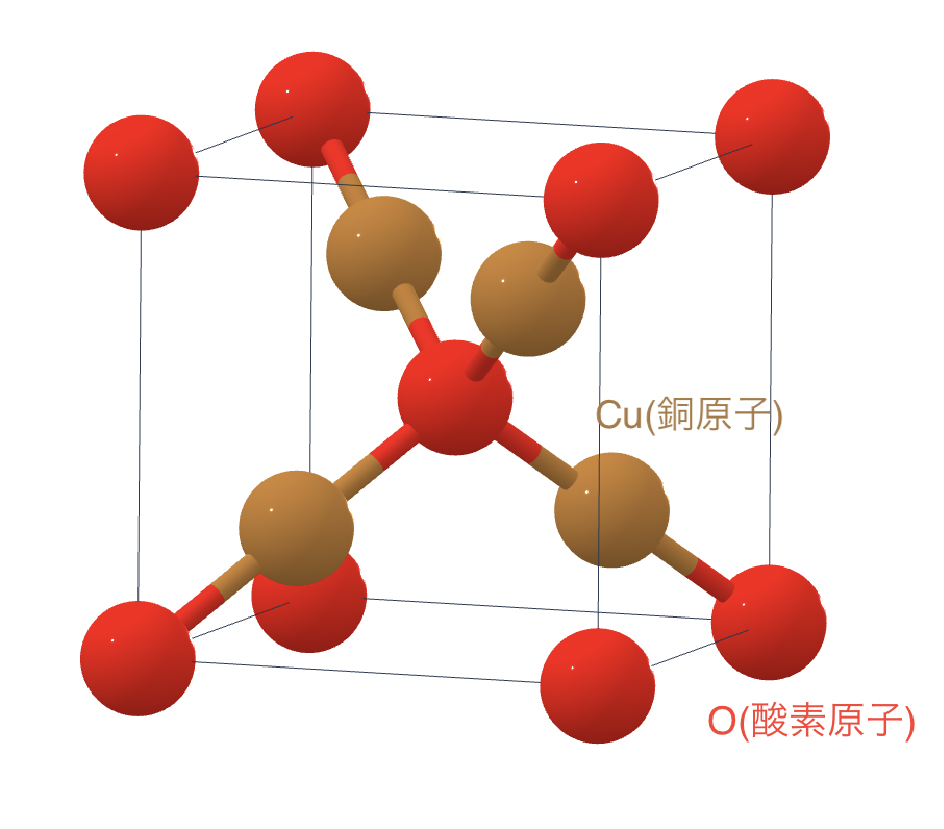
\includegraphics[width=80mm]{Screen_2024-07-02_2.21.43.eps}
\caption{亜酸化銅結晶の単位格子。Materials Explorerを使用した。}
\end{center}
\end{figure}

\subsection{謎}
なぜ亜酸化銅結晶では高密度・低温条件下でも電子正孔液滴が形成されないのか?
亜酸化銅結晶の黄色系列励起子は結合エネルギーが比較的大きく非常に安定な励起子状態であり、放射再結合を通じてエネルギーを逃がしやすい。
Cu2Oは直接遷移型半導体である。
なぜ分子励起子の形成が抑制されているのか?
電子-正孔交換相互作用が大きいため、スピンフリップには高いエネルギーである。
電子と正孔の交換相互作用が大きいため、スピン反転を伴う励起子分子(ビエキシトン)の形成が妨げられます。

\subsection{黄色系列 1s 励起子の光学遷移}

$\Gamma_6^+$ を利用して次のように決まる。

\[
\Gamma_6^+ \otimes \Gamma_7^+ = \Gamma_6^+ \oplus \Gamma_6^- \oplus \Gamma_7^+ \oplus \Gamma_7^-
\tag{2.1}
\]

ここで 3 重に縮退した $\Gamma_7^+$ がオルソ励起子に、$\Gamma_6^+$ がパラ励起子に対応する。オルソ励起子は電子と正孔の交換相互作用によって 12.1 meV のエネルギー分裂が生じている。
$\Gamma_6^+$ 伝導帯の電子は全角運動量 $j$ において $j = 1/2$ のスピン状態 $| \uparrow \rangle$、$| \downarrow \rangle$ で表される。一方 $\Gamma_7^+$ 価電子帯の正孔は 3d 軌道に由来するため、全角運動量 $j = 5/2$ となる。この値電子帯の正孔は $| \uparrow \rangle$、$| \downarrow \rangle$ の状態を 1 つのスピン成分で書き表される。正孔のスピンを下向きと定義している。

\[
\begin{cases}
\text{ortho:} & \begin{cases}
J = 1, J_z = 1 & = | \uparrow e \uparrow H \rangle \\
J = 1, J_z = 0 & = \frac{1}{\sqrt{2}} ( | \uparrow e \uparrow H \rangle - | \downarrow e \uparrow H \rangle ) \\
J = 1, J_z = -1 & = | \downarrow e \uparrow H \rangle \\
\end{cases} \\
\text{para:} & J = 0, J_z = 0 = \frac{1}{\sqrt{2}} ( | \uparrow e \uparrow H \rangle + | \downarrow e \uparrow H \rangle )
\end{cases}
\tag{2.2}
\]

このとき $\Gamma_6^+$ 伝導帯の電子 $| \uparrow e \rangle$、$| \downarrow e \rangle$ の状態は、この状態のワニエ関数と、電子の純スピン関数 $| \uparrow \rangle$、$| \downarrow \rangle$ で書き表すと

\[
| \uparrow e \rangle = \phi_s^c | \uparrow \rangle
\]

である。一方 $\Gamma_7^+$ 価電子帯の正孔 $| H \rangle$ の状態は、ワニエ関数と正孔の純スピン関数 $| \uparrow H \rangle$、$| \downarrow H \rangle$ で表すと

\[
| \uparrow H \rangle = - \frac{1}{\sqrt{3}} \left\{ ( \phi_{yz}^v + i \phi_{zx}^v ) | \uparrow H \rangle + \phi_{xy}^v | \downarrow H \rangle \right\}
\]

\[
| \downarrow H \rangle = - \frac{1}{\sqrt{3}} \left\{ ( \phi_{yz}^v - i \phi_{zx}^v ) | \uparrow H \rangle - \phi_{xy}^v | \downarrow H \rangle \right\}
\]
\paragraph{直接遷移}
始状態と終状態のパリティが異なる時のみ非ゼロとなり、パリティが「同じであるときはその繊維は電気双極子遷移禁制である。黄色系列励起子は4s軌道と3d軌道の組み合わせであり、両方とも波動関数のパリティが偶であるので双極子遷移禁制である。1sパラ励起子に関しては電気四重極子遷移が許容となる。

1sパラ励起子はスピン禁制であるためほとんど発光しない。したがって、パラ励起子の寿命はマイクロ秒程度と長寿命である。この寿命の長さは不純物によって制限されると考えられる。結晶に歪みをかけた場合、黄色系列1sパラ励起子と緑色系列の励起子が混合して四重極子遷移が微弱に許容となる。
\begin{figure}[htbp]
\centering
\includegraphics[width=0.5\textwidth]{Screenshoot_2024-08-18_0.20.28.png}
\caption{直接遷移型のイメージ図}
\label{fig:直接遷移}
\end{figure}

\paragraph{フォノンを介した発光}
パリティが奇のフォノンが関与することで、パリティ保存則が満たされ、1sオルソ励起子の電気双極子遷移が許容される。光学遷移にかかわるのは $\Gamma$ 点近傍で平坦な分散関係を持つ光学フォノンである。オルソ励起子 $\Gamma_5^+$ の双極子遷移 $\Gamma_4^-$ に寄与するフォノンの対称性は、群論の考察から \[ \Gamma_5^+ \otimes \Gamma_4^- = \Gamma_2^- \oplus \Gamma_3^- \oplus \Gamma_4^- \oplus \Gamma_5^- \tag{2.8} \] である。これらの光学フォノンのエネルギーはそれぞれ $\Gamma_2^-: 43 \text{ meV}$、$\Gamma_3^-: 13.5 \text{ meV}$、$\Gamma_4^-: 18.7 \text{ meV}$、$\Gamma_5^-: 11.0 \text{ meV}$ である。 
光学フォノンを介した光学遷移であるオルソ励起子のフォノンサイドバンド発光について述べる。光学フォノンの分散関係は平坦であるため、エネルギー保存則と運動量保存則は次のようになる。
\[ E_0 + \frac{\hbar^2 k^2}{2m^*} = h\nu + E_{\text{phonon}} \tag{2.9} \] \[ \hbar k = hq + \hbar k_{\text{phonon}} \tag{2.10} \] ここで $E_0$ は励起子の静止エネルギー、$m^*$ は励起子の有効質量、$k$ は励起子の波数、$q$ は光の波数、$E_{\text{phonon}}$ は光学フォノンのエネルギー、$k_{\text{phonon}}$ は光学フォノンの波数、$c$ は光速、$h$ はディラック定数である。光学フォノンの分散関係は平坦で、光子の分散関係は直線で近似的に垂直とみなすことができるので、任意の波数ベクトル $k$ をもつ励起子について、エネルギー保存則と運動量保存則の連立方程式は解を持ち、フォノンサイドバンド発光に寄与しうる。
\begin{figure}[htbp]
\centering
\includegraphics[width=0.5\textwidth]{Screenshoot_2024-08-18_0.21.08.png}
\caption{直接遷移型のイメージ図}
\label{fig:直接遷移}
\end{figure}
フォノンを介した吸収についても考える。対称性が$\Gamma_3^-$のLOフォノン放出を介してオルソ励起子を生成する。エネルギー保存則と運動量の保存則の関係式は
\[ E_0 + \frac{\hbar^2 k^2}{2m^*} = h\nu - E_{\text{phonon}} \tag{2.9} \] \[ \hbar k = hq - \hbar k_{\text{phonon}} \tag{2.10} \] 
と書ける。


この励起子が安定化しているのを初めて発見したのが林、勝木らである。
1sオルソ励起子は1sパラ励起子のエネルギーより$ 12.1\text{ meV}$だけ高エネルギーである。


冷却原子系での相互作用の研究はs波散乱長の観点から評価されている。励起子の研究においては理論的にも実験的評価も報告が少ない。

\subsection{歪印加の元での亜酸化銅結晶の性質}
亜酸化銅結晶におけるオルソ励起子からパラ励起子への転換機構はいまだ解明されておらず議論が続いている。オルソ励起子からパラ励起子への転換の実験は 1.5 K 以上の環境で測定されてきた。そのため、1 K以下の温度環境におけるオルソパラ転換について実験的観測が必要といえる。そこで今回の実験ではサブケルビン温度環境下でのオルソパラ転換レートの測定を行うことでオルソパラ転換の物理的機構の検証および解明を目指した。

1s励起子は双極子遷移禁制であり、他の直接遷移型半導体の励起子と比べて長い寿命をもつ。
スピンを反転させる項がないため直接遷移は完全に禁制である。オルソ励起子が転換して生成されるパラ励起子はマイクロ秒程度の寿命をもつ。特殊な対称性を持つLOフォノンを介した間接遷移が微弱ながら許容となる以外には光を吸収放出するメカニズムが存在していない。

\begin{equation}
    \Gamma_{LO} = \Gamma_5^+ \otimes \Gamma_4^- = \Gamma_2^- \oplus \Gamma_3^- \oplus \Gamma_4^- \oplus \Gamma_5^- 
\end{equation}
$\Gamma_2^-$、$\Gamma_3^-$、$\Gamma_4^-$、$\Gamma_5^-$の対称性を持つもの(エネルギーはそれぞれ43 meV、13.5 meV、18.7 meV(79 meV)、11.0 meV)である。
LOフォノンを介した励起子吸収

励起子の発光スペクトルについて。フォノンサイドバンド発光の形状は励起子のもつ熱分布を反映している。
フォノンについては光学フォノン(Optical Phonon)か音響フォノン(Acoustic Phonon)、そして縦波(Longitudinal Wave)か横波(Transverse Wave)で 4 つに分類することができる。
LOフォノン(Longitudinal Optical Phonon、TOフォノン(Transverse Optical Phonon)、LAフォノン(Longitudinal Acoustic Phonon)、TAフォノン(Transverse Acoustic Phonon)に分類される。縦方向音響(LA)モードは $1$ 個、横方向音響(TA)モードは $2$ 個、縦方向光学( LO)モードは $N - 1$ 個、そして横方向光学( TO)モードは $2(N - 1)$ 個存在します。ここで、$N$ は単位格子内の原子の数を表している。\\
1sパラ励起子のボーズ・アインシュタイン凝縮体の性質を調べるためには、光生成されるオルソ励起子からパラ励起子への転換の物理的機構の解明が重要であるといえる。ここではオルソパラ転換レートの温度依存性の実験的評価と提案されてきたスピン転換の物理的機構の提案についてまとめる。

1982年にCaswellらは対称性の議論からLOフォノンとLAフォノンの二つのフォノン過程によるスピン転換のモデルを提案し、温度依存性を再現した。定常状態におけるオルソ励起子とパラ励起子の個数の温度依存性について議論した。
  Caswellらは1つのフォノンを介したスピン転換は禁制であるとして,
$\Gamma_{12}^{-}$のLOフォノンを採用したのが図\ref{fig:exciton_phonon_sideband2}である。
高温領域においては、詳細釣り合いの原理から推論される$\frac{N_0}{N_p} = \frac{U}{D}$となります。一方、低温領域では、$U$の値が$D$に比べて無視できるとすると、$N$は$\frac{G}{D + \gamma_0}$程度になると考えられます。これにより、$D$の値が低下することでオルソ励起子の数が増加することが説明できます。
\begin{figure}[htbp]
\centering
\includegraphics[width=0.5\textwidth]{screenshoot_2024-08-16_21.20.00.png}
\caption{オルソ励起子 $\Gamma^{-}_{12}$ フォノンサイドバンド発光強度の温度依存性。実線は2フォノンモデルによる実験結果のフィッティングであり、破線は詳細吊り合いの原理から計算された2準位モデルによるフィッティングである。}
\label{fig:exciton_phonon_sideband}
\end{figure}
\begin{figure}[htbp]
\centering
\includegraphics[width=0.5\textwidth]{Screen_2024-08-16_21.32.29.png}
\caption{2フォノンモデルによるオルソ励起子からパラ励起子への転換レート(D$_p$)とパラ励起子からオルソ励起子への転換レート(U)の温度依存性}
\label{fig:exciton_phonon_sideband2}
\end{figure}

1983年にWeinerらはオルソ励起子とパラ励起子の発光強度からオルソパラ転換レートを2.5 Kの温度領域で測定した。その結果、オルソ励起子フォノンサイドバンド発光には二つの減衰成分が含まれているのを観測した。温度に依存する早い成分の減衰と温度に依存しない遅い成分の減衰の二つが見られた。一方、パラ励起子のフォノンサイドバンド発光の減衰は温度に依存しない成分のみが見られた。Weinerは単純な2準位モデルからオルソ励起子の早い転換レートはオルソ-パラ転換レートDとオルソ励起子の寿命$\gamma_0$の和であり、実験結果へのフィッティングから$D+\gamma = \alpha + \beta T^\frac{3}{2}(\alpha = 0.4ns^{-1}、\beta = 0.03 ns^{-1}K^{-\frac{1}{2}})$であると求めた。
\cite{Weiner1983}で$T^{-\frac{3}{2}}$の温度依存性を示していることを求めた。
\begin{figure}[htbp]
\centering
\includegraphics[width=0.5\textwidth]{Screenshoot_2024-08-16_22.40.09.png}
\caption{(a)2.5 K(b)35 K(c)48 Kにおいてのオルソ励起子$\Gamma^{-}_{12}$ フォノンサイドバンド発光とパラ励起子$\Gamma^{-}_{25}$フォノンサイドバンド発光の時間発展}
\label{fig:exciton_phonon_sideband2}
\end{figure}
\begin{figure}[htbp]
\centering
\includegraphics[width=0.5\textwidth]{Screenshoot_2024-08-16_23.06.06.png}
\caption{D+$\gamma_o$の温度依存性。丸は実験結果のプロットの点。実線は$\alpha$+$\beta$ T$^\frac{1}{2}$によるフィッティング曲線、破線は二つのフォノンを介したモデルによるフィッティング曲線。}
\label{fig:exciton_phonon_sideband2}
\end{figure}

1990年にSnokeらはオルソ励起子が 1 個のLAフォノンの放出を介してパラ励起子に変化するモデルを提案した \cite{snoke1990}。SnokeらはLAフォノンが大きな波数を持つ場合、対称性の条件は緩和され、一つのLAフォノンを介したスピン転換が許容となると仮定した。この仮定に基づきDとUの値を計算すると¥refであり、低温領域ではTに比例し、高温領域では$T^{\frac{3}{2}}$を超える温度依存性を示した。その結果、Weinerらの実験結果を再現した。
\begin{figure}[htbp]
\centering
\includegraphics[width=0.5\textwidth]{Screenshoot_2024-08-16_23.59.31.png}
\caption{LAフォノンモデルに基づいて計算されたオルソーパラ転換レートDとパラーオルソ転換レートUの温度依存性。}
\label{fig:exciton_phonon_sideband2}
\end{figure}
\begin{figure}[htbp]
\centering
\includegraphics[width=0.5\textwidth]{Screenshoot_2024-08-17_0.01.54.png}
\caption{黒丸はWeinerらによる実験結果のプロット。実線は1LAフォノンモデルによるフィッティング曲線。点線は2フォノンモデルによるフィッティング曲線。$\gamma$ = 0.1 ns$^{-1}$とした。}
\label{fig:exciton_phonon_sideband2}
\end{figure}


Mysyrowiczらは
・Grossらは
低温高密度領域におけるオルソ励起子同士の衝突により2つのパラ励起子が生成されるモデルも提案されてきた。Kubouchi らは

これまでに提案されてきたオルソパラ転換の物理的機構ではオルソパラ転換レートはゼロ温度付近では0に近づくが、実験での観測では有限値をとる。
2004年にJangらはオルソ励起子が 1 個のTAフォノンのみを介してパラ励起子に転換するモデルを提案した。\cite{jang2004}Jangら
2 Kから20 Kまでの温度領域においてパラ励起子とオルソ励起子の減衰を確認した。Jangらはオルソパラ転換のメカニズムとしてTAフォノンの吸収と放出であることを
格子の回転がスピン軌道相互作用を通じてスピン反転を引き起こすという微視的なモデルを提案した。
オルソパラ転換レートの温度依存性や応力依存性から転換の物理的機構としては1個のTAフォノンが関与するものが最も妥当であると考えられる。
オルソパラ転換レート$D$ の温度依存性は
\[D(T) \sim 1 + \frac{2k_B T}{\hbar \omega}\]
$D(T, \Delta) = D(T) \times (1 + 2n)$
である。
\[
H = \frac{2\alpha}{3} \mathbf{L} \cdot \mathbf{S}^h + 2J \mathbf{S}^e \cdot \mathbf{S}^h 
+ b \sum_{i=x,y,z} \epsilon_{ii} \left( 3 L_i^2 - L^2 \right),
\]
$T = 0\,\mathrm{K}$、オルソ励起子の運動量p=0 、フォノンの自然放出のみを考慮してオルソパラ転換レートを計算する。
\begin{align}
\Gamma^{z}_{\mathrm{op}} &= \frac{2 \pi}{\hbar} \int \frac{d^3q}{(2 \pi)^3} \left| \frac{2J \sin \theta}{9} \right|^2 \frac{q \hbar}{2 \rho v} \delta \left( \Delta - \hbar v q - \frac{\hbar^2 q^2}{2m} \right) \\
&= \frac{2J^2}{81(2\pi)^2 \rho v} \int d^3q \, \sin^2 \theta \, q \, \delta \left( \Delta - \hbar v q - \frac{\hbar^2 q^2}{2m} \right)\\
&= \frac{2J^2}{81(2\pi)^2 \rho v} \int_0^\infty dq \int_0^\pi d\theta \int_0^{2\pi} d\phi \, 
q^3 \sin^3 \theta \, \delta \left( \Delta - \hbar v q - \frac{\hbar^2 q^2}{2m} \right)\\
&= \frac{4J^2}{81(2\pi)^2 \rho v} \frac{8\pi}{3} \frac{q_{\Delta}^3}{\left| - \hbar v - \frac{\hbar^2}{m} q_{\Delta}\right|}\\
&= \left( \frac{2J}{9} \right)^2 \frac{q_{\Delta}^3 / 3 \pi \rho v}{\hbar v + \frac{\hbar^2 q_{\Delta}^2}{m'}}
\end{align}
$\hbar q_{\Delta} = -m v \pm \sqrt{m^2 v^2 + 2 m \Delta}$である。途中デルタ関数の性質$\int dq \, f(q) \, \delta(g(q)) = \frac{f(q_0)}{\left| g'(q_0) \right|}$を用いた。
\begin{align*}
m &= 2.6 \, m_e, \quad m_e = 9.11 \times 10^{-31} \, \text{kg}, \\
\rho &= 6.1 \, \text{kg/cm}^3 = 6.1 \times 10^6 \, \text{kg/m}^3, \\
\Delta &= 12.1 \, \text{meV} = 12.1 \times 10^{-3} \times 1.6 \times 10^{-19} \, \text{J}, \\
v &= 1.3 \, \text{km/s} = 1.3 \times 10^3 \, \text{m/s}.
\end{align*}
$m v$と$2 m \Delta$を比較すると:
\[
m v = 3.08 \times 10^{-27} \, \text{kg} \, \text{m/s}, \quad 2 m \Delta = 9.17 \times 10^{-51} \, \text{kg}^2 \, \text{m}^2/\text{s}^2.
\]
と計算でき、
\[
\hbar q_{\Delta} \approx \frac{\Delta}{v}.
\]

よって
\begin{align}
\Gamma^{z}_{\mathrm{op}} = 
\left( \frac{2J}{9} \right)^2 
\frac{2m^2 \Delta}{3 \pi \rho \nu_T \hbar^4}
\end{align}


ここで光生成されたオルソ励起子の運動量が有限である場合を考える。エネルギー保存則と運動量保存の関係式は以下のようになる。
\begin{equation}
\Delta + \frac{\hbar^2 K^2_{\text{ortho}}}{2 m_{\text{ortho}}} = \hbar v k + \frac{\hbar^2 K^2_{\text{para}}}{2 m_{\text{para}}}, \quad
\hbar K_{\text{ortho}} = \hbar k + \hbar K_{\text{para}}.
\end{equation}


\begin{equation}
\Delta + \frac{\hbar^2 \left| \mathbf{K}_{\text{ortho}} \right|^2}{2 m_{\text{ortho}}} = \hbar v |\mathbf{k}| + \frac{\hbar^2 \left| \mathbf{K}_{\text{para}} \right|^2}{2 m_{\text{para}}},
\quad
\hbar \mathbf{K}_{\text{ortho}} = \hbar \mathbf{k} + \hbar \mathbf{K}_{\text{para}}.
\end{equation}
左式を右式に代入すると
\[
\Delta + \frac{\hbar^2 |\mathbf{k}|^2}{2 m_{\text{ortho}}} + \frac{\hbar^2 \mathbf{k} \cdot \mathbf{K}_{\text{para}}}{m_{\text{ortho}}} = \hbar v |\mathbf{k}| + \hbar^2 |\mathbf{K}_{\text{para}}|^2 \left( \frac{1}{2 m_{\text{para}}} - \frac{1}{2 m_{\text{ortho}}} \right)
\]
オルソ励起子とパラ励起子の質量が同じであると仮定する。
\[
\Delta = \hbar v |\mathbf{k}| - \frac{\hbar^2 |\mathbf{k}|^2}{2 m} - \frac{\hbar^2 \mathbf{k} \cdot \mathbf{K}_{\text{para}}}{m}
\]


生成されるオルソ励起子の運動量について考える。励起光のスペクトルの中心波長が \( 607.47 \, \mathrm{nm} \) であり、短波長側の裾野が \( 607.44 \, \mathrm{nm} \) であるので、トラップ底に生成される励起子の運動量は最大で 
\[
7.89 \times 10^{-26} \, \mathrm{kg \, m/s}
\] 
である。フォノンのエネルギー差は \( \Delta = 12.1 \, \mathrm{meV} \) であり、そのときのフォノンの運動量は 
\[
1.48 \times 10^{-24} \, \mathrm{kg \, m/s}
\] 
である。よって、オルソ励起子の運動量は TA フォノンに比べて小さい。エネルギー保存則から、



\[
\frac{\hbar^2 |\mathbf{k}|^2}{2 m} > \frac{\hbar^2 \, \mathbf{k} \cdot \mathbf{K}_{\text{para}}}{m}
\]
より、
\[
\Delta' = \hbar v |\mathbf{k}| + \frac{\hbar^2 |\mathbf{k}|^2}{2 m}
\]
となる。




圧力をかけるとパラ励起子とオルソ励起子のエネルギー差が変動することを考慮すると
\[
D(\Delta) = \left(\frac{2J}{9} + \frac{3(12 - \Delta)}{8} \right)^2 \frac{2m^2 \Delta}{3 \pi \rho \nu_T \hbar^4}
\]

\begin{figure}[htbp]
\begin{center}
\begin{minipage}[b]{0.45\textwidth}
\centering
\includegraphics[width=\textwidth]{Scrennshoot_2024-07-22_175154.png}
\caption{Jangらが提唱したTAフォノンによるオルソパラ転換レートの検証。オルソパラ転換レートの温度依存性。破線はLAフォノンによる転換過程。}
\end{minipage}
\hspace{0.05\textwidth} % space between the figures
\begin{minipage}[b]{0.45\textwidth}
\centering
\includegraphics[width=\textwidth]{ScreenShoot_2024-07-22_174432.jpeg}
\caption{オルソ励起子の寿命の応力依存性。実線はTAフォノンによる転換プロセス。破線はLAフォノンによるプロセス}
\end{minipage}
\end{center}
\end{figure}

オルソ励起子同士の衝突によるパラ励起子の生成も
これらの先行研究では、いずれも2 K以上の温度領域を対象としていた。サブケルビン温度領域で観測される励起子BECの形成過程の理解には、当該温度領域における転換レートの実験的評価とそれによる従来の物理機構の検証が必須となっている。
\subsection{励起子の波動関数}
入射してくる光の対称性(偏光や波数ベクトル)と励起子の包絡関数で決まる対称性が一致しなければ励起子は生成されない。
波動関数についてはWaters1980を参考にした。
1s励起子の包絡関数である。$\Phi^{1s}$は
\[
\Phi^{1s} = \frac{1}{\sqrt{\pi a^\frac{3}{2}}} \exp\left( -\frac{r}{a} \right)
\]
aはボーア半径である。


\[
\psi_{i}^{1s} =
\begin{cases}
\Phi^{1s}_{Y} \cdot \phi_{i}^{1s} & (i = 5, 8, 10, 12) : \text{黄色系列} \\
\Phi^{1s}_{G} \cdot \phi_{i}^{1s} & (i \ne 5, 8, 10, 12) : \text{緑色系列}
\end{cases}
\]

\begin{table}[h!]
    \centering
    \caption{Wave functions and energies of the 4 yellow and 8 green exciton states with orbital quantum numbers \(n\) including Coulomb and spin-orbit interactions.}
    \begin{tabular}{|c|l|c|l|c|}
        \hline
        No. & Exciton & Symmetry & Wave function & Energy \(E^0\) \\ \hline
        $\phi_{12}$ & Singlet Yellow $\Gamma_2$ (paraexciton) 
        & $\Psi_{\Gamma_2}$ 
        & $\Phi_{yn} \left(\frac{1}{\sqrt{12}}\right) \left[Y^{\prime\prime}(\alpha \beta_C + \beta \alpha_C) + 2 Y_2^{-1} \beta \alpha_C - 2 Y_2^{1} \alpha \alpha_C\right]$ 
        & $E_{c}^{yn}$ \\ \hline

        $\phi_5$ & Triplet $\Gamma_5$ $yz$ 
        & $\Psi_{\Gamma_5 yz}$ 
        & $\Phi_{yn} \left(-\frac{i}{\sqrt{12}}\right) \left[Y^{\prime\prime}(\alpha \alpha_C + \beta \beta_C) + 2 Y_2^{-1} \beta \alpha_C - 2 Y_2^{1} \alpha \beta_C\right]$ 
        & $E_{c}^{yn}$ \\ \hline

        $\phi_8$ & Yellow $3\Gamma_5$ (orthoexciton) 
        & $\Psi_{\Gamma_5 xz}$ 
        & $\Phi_{yn} \left(\frac{1}{\sqrt{12}}\right) \left[Y^{\prime\prime}(\beta \beta_C - \alpha \alpha_C) - 2 Y_2^{1} \alpha \beta_C - 2 Y_2^{1} \beta \alpha_C\right]$ 
        & $E_{c}^{yn}$ \\ \hline

        $\phi_{10}$ & & $\Psi_{\Gamma_5 xy}$ 
        & $\Phi_{yn} \left(-\frac{i}{\sqrt{12}}\right) \left[Y^{\prime\prime}(\beta \alpha_C - \alpha \beta_C) - 2 Y_2^{1} \alpha \alpha_C - 2 Y_2^{-1} \beta \beta_C\right]$ 
        & $E_{c}^{yn}$ \\ \hline

        $\phi_3$ & Triplet $\Gamma_4$ $x$ 
        & $\Psi_{\Gamma_4 x}$ 
        & $\Phi_{gn} \left(\frac{i}{\sqrt{8}}\right) \left[Y^{\prime\prime}(\alpha \alpha_C + \beta \beta_C) + Y_2^{1}(\alpha \beta_C + \beta \alpha_C) - Y_2^{-1}(\beta \alpha_C + \alpha \beta_C)\right]$ 
        & $\Delta + E_c^{gn}$ \\ \hline

        $\phi_6$ & Green $\Gamma_4 y$ 
        & $\Psi_{\Gamma_4 y}$ 
        & $\Phi_{gn} \left(\frac{1}{\sqrt{8}}\right) \left[Y^{\prime\prime}(\beta \beta_C - \alpha \alpha_C) + Y_2^{1}(\beta \alpha_C + \alpha \beta_C)\right]$ 
        & $\Delta + E_c^{gn}$ \\ \hline

        $\phi_1$ & $3\Gamma_4$ 
        & $\Psi_{\Gamma_4 z}$ 
        & $\Phi_{gn} \left(\frac{i}{\sqrt{2}}\right) \left(Y_2^{-1} \alpha \alpha_C + Y_2^{1} \beta \beta_C\right)$ 
        & $\Delta + E_c^{gn}$ \\ \hline
    \end{tabular}
\end{table}
\begin{table}[h!]
    \centering
    \caption{Wave functions and energies of the 4 yellow and 8 green exciton states with orbital quantum numbers \(n\) including Coulomb and spin-orbit interactions (continued).}
    \begin{tabular}{|c|l|c|l|c|}
        \hline
        No. & Exciton & Symmetry & Wave function & Energy \(E^0\) \\ \hline
        $\phi_2$ & Doublet $\Gamma_3$ 
        & $\Psi_{\Gamma_1^3}$ 
        & $\Phi_{gn} \left(-\frac{1}{\sqrt{2}}\right) \left(Y_2^{-1} \alpha \alpha_C - Y_2^{1} \beta \beta_C\right)$ 
        & $\Delta + E_c^{gn}$ \\ \hline

        $\phi_{11}$ & Green $2\Gamma_3$ 
        & $\Psi_{\Gamma_3^2}$ 
        & $\Phi_{gn} \left(-\frac{1}{\sqrt{6}}\right) \left[Y^{\prime\prime}(\alpha \beta_C + \beta \alpha_C) + Y_2^{1} \alpha \alpha_C - Y_2^{-1} \beta \beta_C\right]$ 
        & $\Delta + E_c^{gn}$ \\ \hline

        $\phi_4$ & Triplet $\Gamma_5$ $yz$ 
        & $\Psi_{\Gamma_5 yz}$ 
        & $\Phi_{gn} \left(-\frac{i}{\sqrt{24}}\right) \left[Y^{\prime\prime}(\alpha \alpha_C + \beta \beta_C) + 3\left(Y_2^{-1} \alpha \beta_C - Y_2^{1} \beta \alpha_C\right)\right]$ 
        & $\Delta + E_c^{gn}$ \\ \hline

        $\phi_7$ & Green $3\Gamma_5$ 
        & $\Psi_{\Gamma_5 xz}$ 
        & $\Phi_{gn} \left(\frac{1}{\sqrt{24}}\right) \left[Y^{\prime\prime}(\beta \beta_C - \alpha \alpha_C) - 3\left(Y_2^{-1} \alpha \beta_C + Y_2^{1} \beta \alpha_C\right)\right]$ 
        & $\Delta + E_c^{gn}$ \\ \hline

        $\phi_9$ & & $\Psi_{\Gamma_5 xy}$ 
        & $\Phi_{gn} \left(\frac{1}{\sqrt{6}}\right) \left[Y^{\prime\prime}(\beta \alpha_C - \alpha \beta_C) + Y_2^{1} \alpha \alpha_C + Y_2^{-1} \beta \beta_C\right]$ 
        & $\Delta + E_c^{gn}$ \\ \hline
    \end{tabular}
\end{table}


\begin{figure}[htbp]
\begin{center}
\includegraphics[width=100mm]{Screenshoot_2024-08-06_161849.png}
\caption{フォノンの振動モード}
\end{center}
\end{figure}



\[
\begin{array}{|c|c|c|}
\hline
 & \phi_{1}^{1s} ( \Gamma_{4}^{z} ) & \phi_{2}^{1s} ( \Gamma_{3}^{z} ) \\
\hline
\phi_{1}^{1s} & \frac{J_{G}}{2} & 0 \\
\hline
\phi_{2}^{1s} & 0 & \frac{J_{G}}{2} \\
\hline
\end{array}
\]

\[
\begin{array}{|c|c|c|c|}
\hline
 & \phi_{3}^{1s} ( \Gamma_{4}^{x} ) & \phi_{4}^{1s} ( \Gamma_{5}^{y x} ) & \phi_{5}^{1s} ( Y \Gamma_{5}^{y z} ) \\
\hline
\phi_{3}^{1s} & \frac{J_{G}}{2} & 0 & 0 \\
\hline
\phi_{4}^{1s} & 0 & -\frac{5 J_{G}}{6} & \frac{2 \sqrt{2} J}{3} \\
\hline
\phi_{5}^{1s} & 0 & \frac{2 \sqrt{2} J}{3} & -\frac{J_{Y}}{6} \\
\hline
\end{array}
\]

\[
\begin{array}{|c|c|c|c|}
\hline
 & \phi_{6}^{1s} ( \Gamma_{4}^{y} ) & \phi_{7}^{1s} ( \Gamma_{5}^{z x z} ) & \phi_{8}^{1s} ( Y \Gamma_{5}^{z x z} ) \\
\hline
\phi_{6}^{1s} & \frac{J_{G}}{2} & 0 & 0 \\
\hline
\phi_{7}^{1s} & 0 & -\frac{5 J_{G}}{6} & \frac{2 \sqrt{2} J}{3} \\
\hline
\phi_{8}^{1s} & 0 & \frac{2 \sqrt{2} J}{3} & -\frac{J_{Y}}{6} \\
\hline
\end{array}
\]

\[
\begin{array}{|c|c|c|}
\hline
 & \phi_{9}^{1s} ( \Gamma_{5}^{x y} ) & \phi_{10}^{1s} ( Y \Gamma_{5}^{x y} ) \\
\hline
\phi_{9}^{1s} & -\frac{5 J_{G}}{6} & \frac{2 \sqrt{2} J}{3} \\
\hline
\phi_{10}^{1s} & \frac{2 \sqrt{2} J}{3} & -\frac{J_{Y}}{6} \\
\hline
\end{array}
\]

\[
\begin{array}{|c|c|c|}
\hline
 & \phi_{11}^{1s} ( \Gamma_{3}^{2} ) & \phi_{12}^{1s} ( Y \Gamma_{2} ) \\
\hline
\phi_{11}^{1s} & \frac{J_{G}}{2} & 0 \\
\hline
\phi_{12}^{1s} & 0 & \frac{J_{Y}}{2} \\
\hline
\end{array}
\]
亜酸化銅結晶に歪みを書けると対称性が低下して、 $O_h^4$ から $D_{4h}$ に変化する。歪をかけられていない場合パラ励起子はすべての次数において光学応答をしないが、歪をかけられた場合は波動関数に緑色系列が混ざるためにパラ励起子の光学応答が微弱ながら許容となる。光学応答の度合いは応力の大きさに依存する。
このように生成された励起子をトラップするために歪をかけているが、
素過程においての応力が印加された状況について考察していいくのが本研究の重要な点であり、解析を難しくしている点である。
\subsection{励起子BECの先行研究}
1950年にHayashiらは亜酸化銅結晶の離散的な吸収線を発見して、半導体における励起子の存在を発見した。
1970年代には波長可変のレーザーが発明され半導体において高密度に励起子を生成することができるようになった。レーザー光のパワーを調整することで高密度に励起子を生成することができる。固体結晶と熱平衡を保つ環境ので励起子がBEC状態に転移するかどうかは長年の疑問であった。励起子は粒子数が保存されない開放系という特徴をもつ。励起子の寿命は有限であり、寿命以内で環境との接触などにより系全体が熱平衡にあると近似的に見做せる状態(準熱平衡状態)においてのBECが観測できる。これらの励起子でBECが発生するかどうかは冷却原子系との大きな違いである。

励起子の有効質量は電子の質量と同程度の重さであり、他の原子と比べて桁違いに小さい。液体ヘリウム温度領域でのBECが可能であると考えられてきた。
励起子を1s-2p遷移の吸収スペクトルによって1sパラ励起子の温度と密度を正確に評価したところ、1sパラ励起子の二体非弾性散乱による消失が当初予想していたよりも大きく励起子BECの実現が遠のいた。
励起子の密度の評価方法として励起子Lymman分光法が考えられてきた。この実験方法では中赤外領域に生じる内部遷移吸収を利用するものである。

亜酸化銅結晶を超流動ヘリウム温度に冷却することで、励起子BECの研究が盛んに行われました。しかし、パラ励起子同士の非常に大きな非弾性衝突係数のため、この温度領域でのBEC形成は困難であることが分かった。そのため、ヘリウム3冷凍機や希釈冷凍機を使用して、BEC転移密度を下げた温度領域で実験が行わてきた。
結晶中に非一様な歪みを形成して、トラップポテンシャルを形成することにより、パラ励起子が亜酸化銅結晶全体に拡散することなく、ポテンシャルの底に収集される。

励起子自体が励起状態であることやボーズ粒子としてどうふるまうのかは自明ではない。

Yoshiokaら\cite{Yoshioka2011}は$^3\text{He}$冷凍機を用いて、励起子温度を700 mKまで冷却し、パラ励起子の空間分解発光スペクトルの変化の様子を観測した。そして水素原子のBECでも観測された、「緩和爆発」という現象を亜酸化銅結晶でも観測した。このことから亜酸化銅結晶における励起子BECを間接的に観測したと結論づけた。緩和爆発という現象から凝縮体は安定に存在できなかった。

Moritaら\cite{Morita2022}は中赤外光を用いた吸収イメージングの手法を開発し、結晶の3次元トラップに生じた凝縮体の直接的に観測することに成功した。Moritaらは窓つきの希釈冷凍機を用いることでmixing chamber温度64 m Kの結晶温度を保持しつつ、中赤外で光学アクセス可能な実験をおこなった。しかし、ボーズアインシュタイン凝縮体を構成する励起子の割合が理想的なBose気体から期待される 100 \%に比べて 1.6 \%に留まるといった、未解明の点が残った。また、励起子間には弱い斥力が働いていることがわかった。量子系のコヒーレンス、デコヒーレンスの仕組み

\begin{figure}[htbp]
\begin{center}
\includegraphics[width=100mm]{Screenshoot_2024-08-16_4.31.11.png}
\caption{中赤外吸収イメージングによって得られたパラ励起子の空間密度分布。}
\end{center}
\end{figure}


また、励起子系は有限の寿命による消滅と定常光による光生成が繰り返される非平衡系であるため、励起子BECは非平衡量子統計力学の解明の実験として考えられている。

冷却レートについて。結晶の格子系を冷却することで熱接触により励起子温度を冷やされる。あつい励起子はフォノンとの相互作用によって冷却されていく。LAフォノンによる冷却。TAフォノンはLAフォノンと比べて音速が小さいので小さい運動量をもつ励起子と散乱することができる。歪みがかけられていない場合、対称性の観点からLAフォノンによる冷却のみ可能であるが、歪みをかけるとTAフォノンによる冷却も可能になる。
Yoshiokaらによれば励起子の有効質量は$m_{1s-para} = 2.4\pm0.34$ $m_{0}$である。
\subsection{亜酸化銅結晶の特徴}
\paragraph{太陽電池}
太陽エネルギーを活用するための低コストの太陽電池

\paragraph{リュードベリ励起子}
リュードベリ励起子は、高い主量子数を持つ励起状態の電子と正孔の対が結合したもので、巨大なボーア半径と長い寿命を特徴とします。大きな電気双極子モーメントを有するため、外部電場や磁場に対して敏感であり、量子情報系の研究や高精度分光技術に用いられる可能性があります。実験的には、超高品質な半導体材料とレーザー分光を組み合わせることで、その特性を詳細に解析する試みが進められています。

\paragraph{薄膜}
うすい
\newpage

\newpage
\section{実験機材の説明}
\subsection{観測系の装置}
\subsection*{亜酸化銅結晶試料}
今回の実験で用いたのはナミビア産の天然亜酸化銅結晶である。
人工的に作り出すことはできるが、不純物や高純度性の観点から天然結晶を用いている。
結晶は大きさは5.3\,\text{mm} \times 5.3\,\text{mm} \times 8.0\,\text{mm}の寸法の直方体である。

\subsection*{希釈冷凍機}
\begin{figure}[htbp]
\begin{center}
\includegraphics[width=100mm, angle=270]{IMG_8626.jpeg}
\caption{無冷媒希釈冷凍機}
\end{center}
\end{figure}
結晶の冷却にはOxford Instruments社の無冷媒希釈冷凍機(DR-400)を用いている。
希釈冷凍機とは$^3$Heと$^4$Heの混合液の相分離におけるエントロピー差を利用した冷却に実現している。
この冷凍機では、長期間にわたり低温環境を安定的に維持することが可能であり、設計上無冷媒であることからメンテナンスフリーであり数ヶ月にわたる運転が可能である。
理論上では、無限に低い温度環境を維持することが可能であるが、実際には外部からの熱流入が最低温度の限界を決定する。
電気抵抗に電流を流すことで熱を発生させ、冷却対象の温度を制御することができる。
DR-400には、励起光やプローブ光を入射するために窓が付けられている。
窓の設計は低温環境を維持するために様々な工夫がなされている。
温度はどこまでを維持れるんだっけ?希釈冷凍機では数十mKまでを達成することができるが、今回の実験のセットアップでは最低温度64 mKが達成可能である。
運転中に混入する不純ガスは、希釈冷凍機の性能を低下させる原因となる。
これを防ぐために外部でLN2 trapを使用することで不純ガスを回収する。
希釈冷凍機のサンプルステージには、不均一な応力印加用のレンズ(圧力印加用レンズ)と微弱な励起子の集光用のレンズ(発光観測用のレンズ)が設置されている。
それぞれ電圧を印加することで精密な位置操作を実現するピエゾを用いている。

\subsection*{複屈折の観測}
ピエゾ素子に電圧をかけること
材料が異方性を持つために、光が二つの異なる経路に分かれて進む現象のことである。
それぞれ二つの波がそれぞれ異なる屈折率をもつ。
ニコル配置
この実験ではピエゾ素子をねじまきがついている回転盤につけることによって上下の運動を制御することができる。
という値をもつ。

\subsection{エネルギーシフトの計算方法}
\begin{align}
    u(y, z, r_0) &= \frac{1}{2} \left( y^2 + z^2 - r_0^2 + \sqrt{(y^2 + z^2 - r_0^2)^2 + 4 r_0^2 z^2} \right) \\
    \sigma_{xx}(y, z, r_0, p_0, \nu) &= -p_0 \left[
        \begin{cases} 
            0 & (y = 0) \\
            \frac{(1 - 2\nu) r_0^2}{3 (y^2 + \epsilon)} \left( 1 - \left( \frac{z}{\sqrt{U}} \right)^3 \right) & (y \neq 0)
        \end{cases}
        + \frac{z}{\sqrt{U}} \left( 2\nu + \frac{(1 - \nu) U}{r_0^2 + U + \epsilon} - \frac{(1 + \nu) \sqrt{U}}{r_0} \arctan \left( \frac{r_0}{\sqrt{U}} \right) \right)
    \right] \\
    \sigma_{yy}(y, z, r_0, p_0, \nu) &= -\sigma_{xx} - \sigma_{zz} + 2 p_0 (1 + \nu) \frac{z}{\sqrt{U}} \left(
        -1 + \frac{\sqrt{U}}{r_0} \arctan \left( \frac{r_0}{\sqrt{U}} \right)
    \right) \\
    \sigma_{zz}(y, z, r_0, p_0) &= -p_0 \frac{\left( \frac{z}{\sqrt{U}} \right)^3 r_0^2 U}{U^2 + r_0^2 z^2} \\
    \sigma_{yz}(y, z, r_0, p_0) &= -p_0 \frac{y z^2 r_0^2 \sqrt{U}}{(U^2 + r_0^2 z^2)(r_0^2 + U)} \\
    \sigma_{xy}(y, z, r_0, p_0) &= 0 \\
    \sigma_{zx}(y, z, r_0, p_0) &= 0
\end{align}

$p_0$ は接触部分にかかる圧力を表し、
\begin{equation}
p_0 = \frac{3 F_0}{2 \pi r_0^2}
\end{equation}

という値を持つ。他の値については

\begin{equation}
\left\{
\begin{aligned}
F_0 &: \text{加える力} \\
R &: \text{結晶を押す物質の曲率半径} \\
E &: \text{結晶のヤング率} \\
\nu &: \text{結晶のポアソン比} \\
E_{\text{push}} &: \text{結晶を押す物質のヤング率} \\
\nu_{\text{push}} &: \text{結晶を押す物質のポアソン比}
\end{aligned}
\right.
\end{equation}

\begin{align*}
F_0 &= 160~\text{N} && \text{外力} \\
R &= 15.57 \times 10^{-3}~\text{m} && \text{曲率半径} \\
E &= 237 \times 10^{8}~\text{Pa} && \text{結晶のヤング率} \\
\nu &= 0.445 && \text{結晶のポアソン比} \\
E_{\text{push}} &= 801 \times 10^{8}~\text{Pa} && \text{結晶を押す材料のヤング率} \\
nu_{\text{push}} &= 0.208 && \text{結晶を押す材料のポアソン比}
\end{align*}

加える力 \( F_0 \) は外力の大きさとして \( 160~\text{N} \) であり、結晶を押す物質の曲率半径 \( R \) は \( 15.57 \times 10^{-3}~\text{m} \) です。また、結晶のヤング率(Young's modulus) \( E \) は \( 237 \times 10^{8}~\text{Pa} \)、ポアソン比(Poisson's ratio) \( \nu \) は \( 0.445 \) です。さらに、結晶を押す物質のヤング率 \( E_{\text{push}} \) は \( 801 \times 10^{8}~\text{Pa} \)、ポアソン比 \( \nu_{\text{push}} \) は \( 0.208 \) となっています。


応力テンソルから歪テンソルからの変換は弾性コンプライアンス定数を通して関連づけられる。
\begin{equation}
\begin{pmatrix}
    \epsilon_{xx} \\
    \epsilon_{yy} \\
    \epsilon_{zz} \\
    \epsilon_{xy} \\
    \epsilon_{yz} \\
    \epsilon_{zx}
\end{pmatrix} = 
\begin{pmatrix}
    S_{11} & S_{12} & S_{12} & 0 & 0 & 0 \\
    S_{12} & S_{11} & S_{12} & 0 & 0 & 0 \\
    S_{12} & S_{12} & S_{11} & 0 & 0 & 0 \\
    0 & 0 & 0 & \frac{S_{44}}{2} & 0 & 0 \\
    0 & 0 & 0 & 0 & \frac{S_{44}}{2} & 0 \\
    0 & 0 & 0 & 0 & 0 & \frac{S_{44}}{2}
\end{pmatrix}
\begin{pmatrix}
    \sigma_{xx} \\
    \sigma_{yy} \\
    \sigma_{zz} \\
    \sigma_{yz} \\
    \sigma_{zx} \\
    \sigma_{xy}
\end{pmatrix}
\end{equation}

以下に歪み(Strain)計算に使用する材料定数を示します。
結晶の弾性コンプライアンス定数として、\( S_{11} = 4.17 \times 10^{-11}~\text{Pa}^{-1} \)、\( S_{12} = -1.94 \times 10^{-11}~\text{Pa}^{-1} \)、および \( S_{44} = 8.26 \times 10^{-11}~\text{Pa}^{-1} \) が得られています。

材料に歪みが加わることでハミルトニアンが変化します。歪みの大きさが小さい場合、この変化を摂動として扱うことが可能です。摂動ハミルトニアン $H_{\text{deformation}}$ は、歪テンソルおよびデフォーメーションポテンシャルの定数によって表現されます。
\begin{align}
H_{\text{deformation}} &= a \, \operatorname{Tr}\, \epsilon 
- 3b \left[ \left(L_z^2 - \frac{1}{3} L^2 \right)\epsilon_{zz} 
+ \left(L_y^2 - \frac{1}{3} L^2 \right)\epsilon_{yy} 
+ \left(L_x^2 - \frac{1}{3} L^2 \right)\epsilon_{xx} \right] \\
&\quad - \sqrt{3}\,d \left[ (L_z L_y + L_y L_z)\epsilon_{xy} 
+ (L_y L_x + L_x L_y)\epsilon_{yx} 
+ (L_z L_x + L_x L_z)\epsilon_{zx} \right]
\end{align}

ここで、$a$ は等方的なデフォーメーションポテンシャル、$b$ と $d$ はそれぞれ剪断変形に関連するポテンシャル、$L$ およびその成分 $L_x$, $L_y$, $L_z$ は角運動量演算子を示します。
この摂動ハミルトニアンに対して、オルソ励起子およびパラ励起子に対する二次の摂動まで考慮することで、歪みによるエネルギーの変動を精密に評価できます。
三重に縮退したオルソ励起子に対する一次摂動ハミルトニアンは以下のように記述されます。固有関数を解析することで、縮退が解消されたオルソ励起子のエネルギー準位を導出できます。(ここで、$\eta = \frac{4|a|}{E_{\text{so}}}$ と定義します)

\begin{equation}
H_1^{\text{ortho}} = a \, \text{Tr}\,e \begin{pmatrix}
1 & 0 & 0 \\
0 & 1 & 0 \\
0 & 0 & 1 \\
\end{pmatrix} + \eta \begin{pmatrix}
b(2e_{xx} - e_{yy} - e_{zz}) & \sqrt{3d}\,e_{xy} & \sqrt{3d}\,e_{zx} \\
\sqrt{3d}\,e_{xy} & b(2e_{yy} - e_{xx} - e_{zz}) & \sqrt{3d}\,e_{yz} \\
\sqrt{3d}\,e_{zx} & \sqrt{3d}\,e_{yz} & b(2e_{zz} - e_{xx} - e_{yy}) \\
\end{pmatrix}
\end{equation}

一方、パラ励起子に対する一次摂動によるエネルギー変化は以下のように表されます。
\begin{equation}
\Delta E_1^{\text{para}} = a \, \text{Tr}\,e
\end{equation}

さらに、二次摂動によるエネルギー変動 $\Delta E_2$ を計算すると、オルソ励起子およびパラ励起子の両方に対して同一の値が得られます。これは価電子帯のエネルギーが上昇するため、励起子のエネルギーは負方向にシフトします。
\begin{equation}
\Delta E_2 = \frac{(3b)^2}{E_{\text{so}}} \left\{(e_{xx} - e_{yy})^2 + (e_{yy} - e_{zz})^2 + (e_{zz} - e_{xx})^2 \right\} + \frac{2(3d)^2}{E_{\text{so}}} \left(e_{xy}^2 + e_{yz}^2 + e_{zx}^2\right)
\end{equation}

デフォーメーションポテンシャルの具体的な値は以下の通りとします。
結晶のエネルギーパラメータとして、\( a = -1.18 \, \text{eV} \)、\( b = -0.40 \, \text{eV} \)、および \( d = 0.31 \, \text{eV} \) です。また、交換相互作用定数は \( J = 23.8 \, \text{eV} \)、スピン軌道結合エネルギーは \( E_{\text{so}} = 131 \, \text{meV} \) です。さらに、無次元パラメータ \( \eta \) は \( \eta = \frac{4|a|}{E_{\text{so}}} = 0.727 \) となります。


これらの式を計算することで1s励起子(パラ/オルソ)のエネルギー変移 $\Delta E_1^{\text{para/ortho}} - \Delta E_2$ を求めることができる。

Trauernichit1986によると[100]方向



\subsection{励起光の実験装置}
\subsubsection*{再生増幅機}
励起子の生成するための励起光の発生源として再生増幅機(Coherent INc 社製 Libra HE)を使用している。
中心波長が800nmであり、パルス幅100 fsの高強度のパルス光を生成し、繰り返し周波数は1 kHzである。
再生増幅器はシード光(Vitesse)が初期の光パルスを提供し、キャビティ内で増幅媒体を何度も通過することでパルスが増幅される。十分に増幅された段階でパルスをキャビティ外に取り出す。
ポンプレーザー(Evolution-15)がシードレーザーを増幅する、最後にストレッチャー/コンプレッサーがパルス広がりを調整した後、強力なパルスに圧縮する。

\subsubsection*{光パラメトリック増幅器(OPA)}
再生増幅機で生成された光の中心波長を調整するためにOPA(Optical Parametric Amplifer: Light Conversion社 TOPAS)を用いた。
OPAでは入力されたシグナル光が非線形結晶を通過する際、ポンプ光との相互作用によシグナル光が増幅され、それと同時にアイドル光が生成される。
アイドル光は、信号光とエネルギーを共有する形で増幅を助ける役割を果たす。

\subsubsection*{CCDカメラ}
CCDカメラは光子を電荷に変換し、その電荷を転送して最終的にデジタル信号として読み出す半導体素子である。

\subsubsection*{分光器}
Spectra Pro-500iモデルを用いた。
回折格子、プリズム
コリメータ: 入射光を平行光にするためのレンズまたはミラー。
スペクトルの波長校正に関してはネオン輝線を用いた。
観測された3つのスペクトルに
参考値としては$609.616\mathrm{nm}$、$614.306\mathrm{nm}$、$609.616\mathrm{nm}$、$616.359\mathrm{nm}$のネオンの輝線を用いた。

\subsubsection*{EMCCDカメラ}
EMCCDカメラは電子増幅技術(Electron Multiplication)を利用して微弱な光信号を高感度で検出するカメラである。
各電子が他の電子を励起して数十倍から千倍に増幅される。
EMCCDカメラには1ピクセルあたり$16 \, \mu \text{m} \times 16 \, \mu \text{m}$の大きさのCCD素子が1600$\times$200で並んでいる。
200ピクセルは分光器に集光された光の縦方向の情報に対応する。

\subsubsection*{ICCDカメラ}

ICCDカメラはフォトカソードとMCPがある。高速現象観測、パルスレーザー測定に
微弱な励起光を検出するためにICCDカメラ(Andor社製 iStar)を用いた。
このICCDカメラでは1ピクセルあたり$13 \, \mu \text{m} \times 13 \, \mu \text{m}$の大きさのCCDが$1024 \times 1024$並んでいる。
externalモードをかけることでゲートをかけるタイミングは外部信号の立ち上がりまたは立ち下がりを時間原点として同期させることができる。

\subsection{全体の実験装置の概略}
実験装置のがいきこ

\subsection{エネルギーシフトの計算方法}

\input{chapter5.tex}
\newpage
\section{まとめと展望}

\newpage
\section{まとめ}
非平衡統計力学の知識とか?二体衝突のLindblad 方程式。薄膜の亜酸化銅、Rydberg励起子。
\newpage


\begin{thebibliography}{9}

\bibitem{inui1980}
犬井鉄郎・田辺行人・小野寺嘉孝, 応用群論(増補版) -群表現と物理学-, 裳華房 (1980)

\bibitem{Pethick2008}
Pethick, C. J., and H. Smith. Bose-Einstein Condensation in Dilute Gases. Illustrated edition. New York: Cambridge University Press, 2008.

\bibitem{Yu2010}
Yu, P. Y.,  Cardona, M. (2010). Fundamentals of Semiconductors: Physics and Materials Properties (4th ed.). Springer.

\bibitem{Clau2012}
Claus F.Klingshirn. Semiconducter Optics. Springer(2012)

\bibitem{Caswell1982}
Caswell, N., and P. Y. Yu. "Physical Origin of the Anomalous Temperature Dependence of the 1S Yellow Exciton Luminescence Intensity in Cu2O." Physical Review B 25, no. 8 (1982): 
\href{https://journals.aps.org/prb/abstract/10.1103/PhysRevB.25.5519}{https://journals.aps.org/prb/abstract/10.1103/PhysRevB.25.5519}

\bibitem{Weiner1983}
Weiner, J. S., N. Caswell, P. Y. Yu, and A. Mysyrowicz. "Ortho- to Para-exciton Conversion in Cu2O: A Subnanosecond Time-resolved Photoluminescence Study." \textit{Solid State Communications} 46, no. 2 (1983)
\href{https://www.sciencedirect.com/science/article/pii/0038109883905884}{https://www.sciencedirect.com/science/article/pii/0038109883905884}

\bibitem{snoke1990}
D. W. Snoke, D. P. Trauernicht, and J. P. Wolfe,
``Mechanism of orthoexciton-to-paraexciton conversion in Cu2O,''
\textit{Physical Review B}, vol. 41, no. 8, pp. 5266, 1990.
\href{https://journals.aps.org/prb/abstract/10.1103/PhysRevB.41.5266}{https://journals.aps.org/prb/abstract/10.1103/PhysRevB.41.5266}

\bibitem{jang2004}
J. I. Jang, K. E. O’Hara, and J. P. Wolfe,
``Spin-exchange kinetics of excitons in Cu$_2$O: Transverse acoustic phonon mechanism,''
\textit{Physical Review B}, vol. 70, 195205, 2004.
\href{https://journals.aps.org/prb/abstract/10.1103/PhysRevB.70.195205}{https://journals.aps.org/prb/abstract/10.1103/PhysRevB.70.195205}

\bibitem{Morita2022}
Y. Morita, K. Yoshioka and M. Kuwata
Gonokami, Nat. Commum. 13, 5388 (2022)

\bibitem{Trauernicht1986}
D. P. Trauernicht, J. P. Wolfe,  Physical Review B 33, 8506 (1986): 
\href{https://journals.aps.org/prb/abstract/10.1103/PhysRevB.33.8506}{\textbf{https://journals.aps.org/prb/abstract/10.1103/PhysRevB.33.8506}}


\bibitem{Yoshioka2011}
K. Yoshioka, E. Chae and M. KuwataGonokami, Nat Commun 2, 328 (2011).

\bibitem{Akiyama}
秋山由洸、2024年度卒業論文
\end{thebibliography}

\newpage
\section{謝辞}
ありがとうございました。


\appendix
\section{冷却方法}
$^3$He-$^4$He混合液を用いた希釈冷凍機の技術により低温環境においての実験が進められてきた。ヘリウムを使うことで$\text{mK}$までの超低温を定常的に保つことができる。

核断熱消磁を用いると
\begin{table}[htbp]
\centering
\begin{tabular}{l|ccccccccc}
\toprule
& \( E \) & \( 8C_3 \) & \( 6C_2 \) & \( 6C_4 \) & \( 3C'_2 \) & \( 8S_6 \) & \( 6\sigma_h \) & \( 6S_4 \) & \( 3\sigma_d \) \\
\midrule
\( A_{1g} \) & 1 & 1 & 1 & 1 & 1 & 1 & 1 & 1 & 1 \\
\( A_{2g} \) & 1 & 1 & -1 & 1 & -1 & 1 & 1 & 1 & -1 \\
\( E_g \) & 2 & -1 & 0 & 2 & 0 & 2 & -1 & 0 & 2 \\
\( T_{1g} \) & 3 & 0 & -1 & -1 & 1 & 3 & 0 & -1 & -1 \\
\( T_{2g} \) & 3 & 0 & 1 & -1 & -1 & 3 & 0 & -1 & -1 \\
\( A_{1u} \) & 1 & 1 & 1 & 1 & 1 & -1 & -1 & -1 & -1 \\
\( A_{2u} \) & 1 & 1 & -1 & 1 & -1 & -1 & -1 & -1 & 1 \\
\( E_u \) & 2 & -1 & 0 & 2 & 0 & -2 & 1 & 0 & 2 \\
\( T_{1u} \) & 3 & 0 & -1 & -1 & 1 & -3 & 0 & 1 & -1 \\
\( T_{2u} \) & 3 & 0 & 1 & -1 & -1 & -3 & 0 & 1 & 1 \\
\bottomrule
\end{tabular}
\caption{Character Table for the \( O_h \) Point Group}
\label{tab:Oh}
\end{table}


\end{document}
